\documentclass[12pt]{report}
\usepackage{fancyhdr}
\usepackage[a4paper]{geometry}
\usepackage[myheadings]{fullpage}
\usepackage{lastpage}
\usepackage{graphicx, wrapfig, subcaption, setspace, booktabs}
\usepackage[T1]{fontenc}
\usepackage[font=small, labelfont=bf]{caption}
\usepackage{fourier}
\usepackage[protrusion=true, expansion=true]{microtype}
\usepackage[english]{babel}
\usepackage{sectsty}
\usepackage{url, lipsum}
\usepackage{float}
\usepackage{listings}
\usepackage[T1]{fontenc}
\usepackage{lmodern}

\newcommand{\HRule}[1]{\rule{\linewidth}{#1}}
\onehalfspacing
\setcounter{tocdepth}{5}
\setcounter{secnumdepth}{5}


% header and footer

\pagestyle{fancy}
\fancyhf{}
\setlength\headheight{15pt}
\fancyhead[L]{Part 1: Web Application Vulnerabilities - 1}
\fancyhead[R]{Security Insider Lab II}
\fancyfoot[R]{Page \thepage\ of \pageref{LastPage}}

% Title page

\begin{document}
	
	\title{ \normalsize \textsc{Lab Report}
			\\ [2.0cm]
			\HRule{0.5pt} \\
			\LARGE \textbf{\uppercase{Security Insider Lab II \\
			Part 1: Web Application Vulnerabilities - 1}}
			\HRule{2pt} \\ [0.5cm]
			\normalsize \vspace*{5\baselineskip}}
	\date{03-05-2017}
	\author{
			Mohammad Saiful Islam \\
			Abhijeet Patil }
	\maketitle
	\newpage
		
		
	\section*{Exercise 1: Setup}
	\paragraph*{1.} {\bf On your Linux machine install apache2, PHP, MySQL and phpmyadmin.}\\ 
	Host machine was used as client and a virtual machine was used as sever for the task. Ubuntu Mate 17.04 was installed in the virtual machine and required packages are installed using following commands:\\
	For apache2: {\fontfamily{qcr}\selectfont
	sudo apt-get install apache2}\\
	For PHP:
	{\fontfamily{qcr}\selectfont
	sudo add-apt-repository ppa:ondrej/php\\
	sudo apt-get update\\
	sudo apt-get install php7.0 php5.6 php5.6-mysql php-gettext php5.6-mbstring php-mbstring php7.0-mbstring php-xdebug libapache2-mod-php5.6 libapache2-mod-php7.0}\\
	After installing, we will choose php5.6 since php7.0 are using different module than the given web application. Command to perform that:\\
	{\fontfamily{qcr}\selectfont
	sudo a2dismod php7.0 ; sudo a2enmod php5.6 ; sudo service apache2 restart}\\
	For Mysql:
	{\fontfamily{qcr}\selectfont
	sudo apt-get install mysql-server}\\
	For phpmyadmin: 
	{\fontfamily{qcr}\selectfont 
	sudo apt-get install phpmyadmin apache2-utils}\\
	We have to add phpmyadmin to the apache configuration. To do that we have to edit {\tt /etc/apache2/apache2.conf}, and add following line. \\
	{\tt Include /etc/phpmyadmin/apache.conf}
	
	\paragraph*{2.} {\bf Download the zipped file of the Vulnerable Bank web application and extract it to your web server. }\\
	We have downloaded the vBank.zip file and extracted to {\tt /var/www/html/} folder. That is the default location where apache will find the application.\\
	
	\paragraph*{3.} {\bf The configuration is located under ./etc/config.php.}\\
	We edit this file to connect to our mysql server at the ''access to database'' section according to the following.\\
	\begin{figure}[H]
		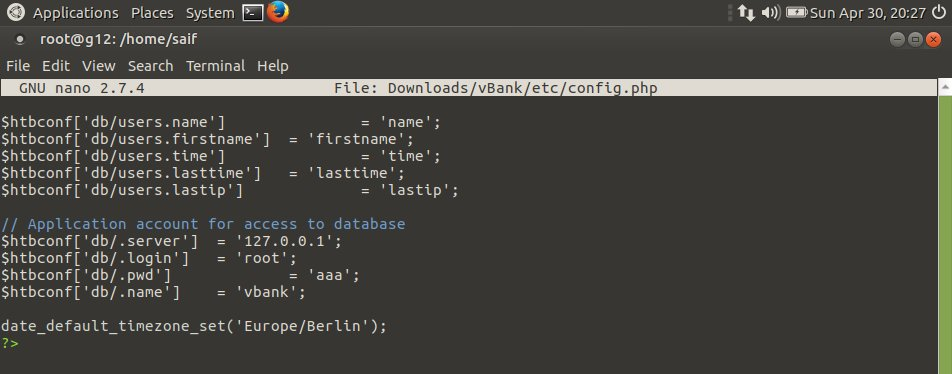
\includegraphics[width=0.75\textheight]{images/config.jpg}
		\caption{config.php}
		\label{fig1:config.php}
	\end{figure}
	
	\paragraph*{4.}	{\bf From phpmyadmin import the file ''vbank.sql'' to setup the database and tables in MySQL}\\
	
	To perform this, In the browser we have entered this: {\tt localhost/phpmyadmin}, then we logged in using credentials. we created a database named 'vbank'. In that database we import the given sql file, and with the phpmyadmin functionality, the database will be created and thus our system will be ready for the application.
	
	\begin{figure}[H]
		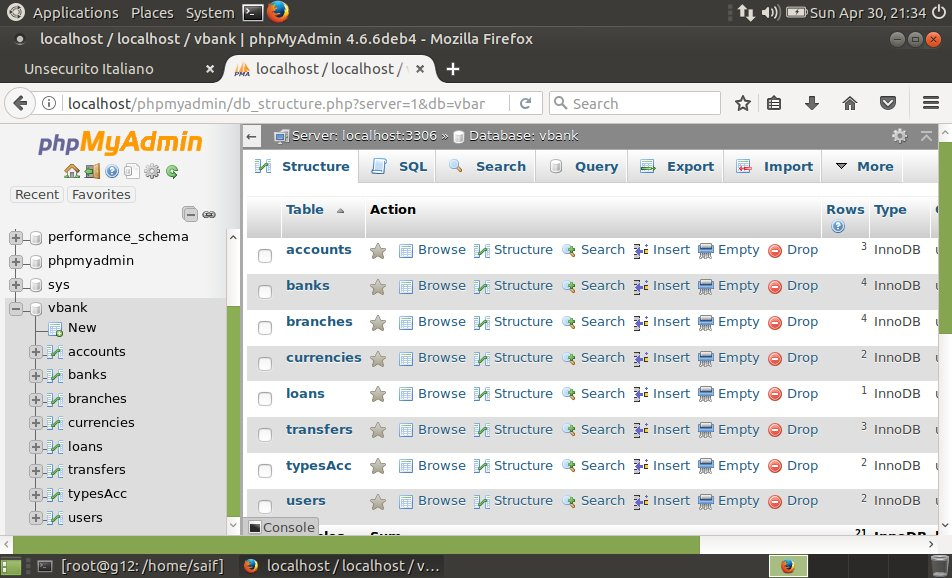
\includegraphics[width=0.75\textheight,height=0.35\textheight]{images/phpmyadmin.jpg}
		\caption{phpmyadmin database}
	\end{figure}
	
	\paragraph*{5.} {\bf Test if the application works from your web browser}\\
	In browser's address bar, when we enter {\tt localhost/vBank/htdocs}, the application will start at it's first page.
	\begin{figure}[H]
		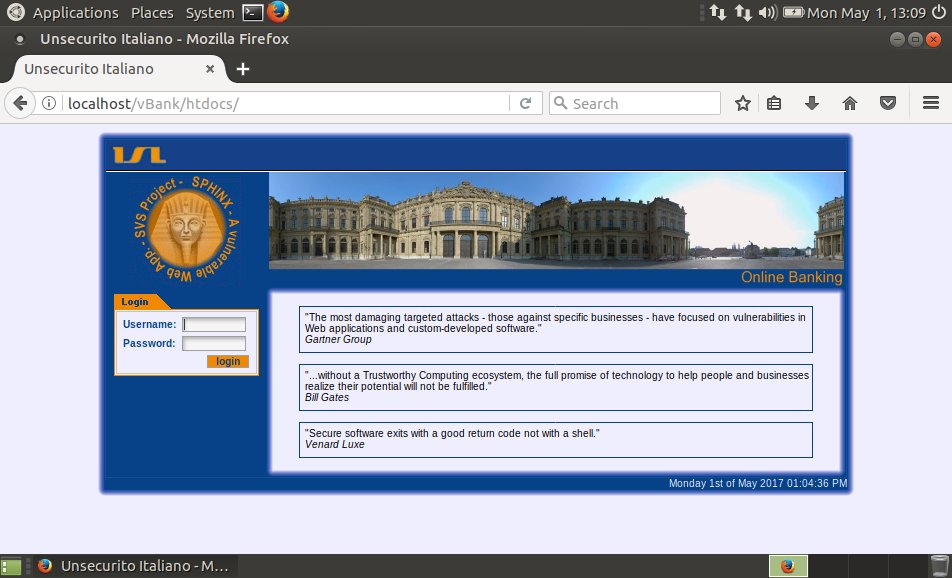
\includegraphics[width=0.75\textheight]{images/apprunning.jpg}
		\caption{vBank application running}
	\end{figure}	
	
	
	\newpage
	
	\section*{Exercise 2: Client/Server Side Scripting}
	
	\paragraph*{1.} {\bf Identify a mechanism which protects the login process (not on the server) and briefly describe the general security problem with this implementation.}\\
	
	On the client machine, using standard firefox browser, when we access to the web app, and try to use some special character as input in the username or password field, it shows an error, saying that only letter and numbers are allowed as valid character.

	\begin{figure}[H]
		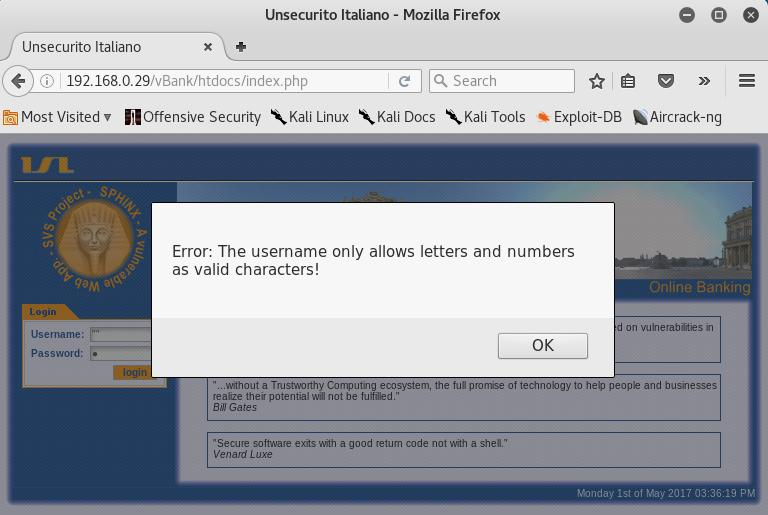
\includegraphics[width=0.75\textheight]{images/javascripterror.jpg}
		\caption{error that restrict to use valid valid character only}
	\end{figure}
	
	It means, on the client side, the app has input validation mechanism, which is typically a javascript code.\\
	Although it is good to have some validation, the security problem is, it is a client side mechanism, and any client-side control can be manipulated by client aka attacker. Just observing the warning, an attacker can have the knowledge of the presence of client-side script, and plan for workaround.
	
	\paragraph*{2.} {\bf List the steps a client could use to circumvent this restriction. Test your approach. Make sure it works.}\\
	There could be several option to circumvent the restriction. Some is stated below.
	\begin{itemize}
		\item JavaScript can be disabled in the browser. Although where there is javascript for input validation, form might require that.
		\item The whole page can be downloaded and altered the source code, and run again in the browser.
		\item Using bypassing tools like Burpsuite.
		\item Encoding attack commands/codes in the website url.
	\end{itemize}
	\paragraph*{3.} {\bf Propose a better solution by providing commented source code.}\\
		The validation should also be in the server side. Before connecting to the database and executing query, the following code can be used to validate incoming string.
	
	\begin{lstlisting}
	/*function isValid($text){
		if (preg_match('/[^a-zA-Z0-9\d]/', $text))
		{
			Return false;	
		}
		Return true;*/
	\end{lstlisting}
	
	\newpage
	
	\section*{Exercise 3: SQL Injection}
	
	\paragraph*{1.} {\bf Find a query to enter the system (without manipulating the data used by the webapplication, you should get access on behalf of another user). Show this query and briefly explain it using the source code at hand.}\\
	
	From client machine, we have tried to exploit by putting special character through username or password field, it did not work because there is a client side defense mechanism which rejects special character. For sql injection, it is necessary to send queries, which always contains special characters.\\
	Another way to perform sql injection is embedded to the url. This type of sql injection is called 'blind' sql injection attack.\\
	First we inspect the index page. In firefox, right click and select 'Inspect Element', another panel will be opened at the bottom of the window, where we select 'network' tab. now if we simply press login, the inspector will show as follows:
	\begin{figure}[H]
		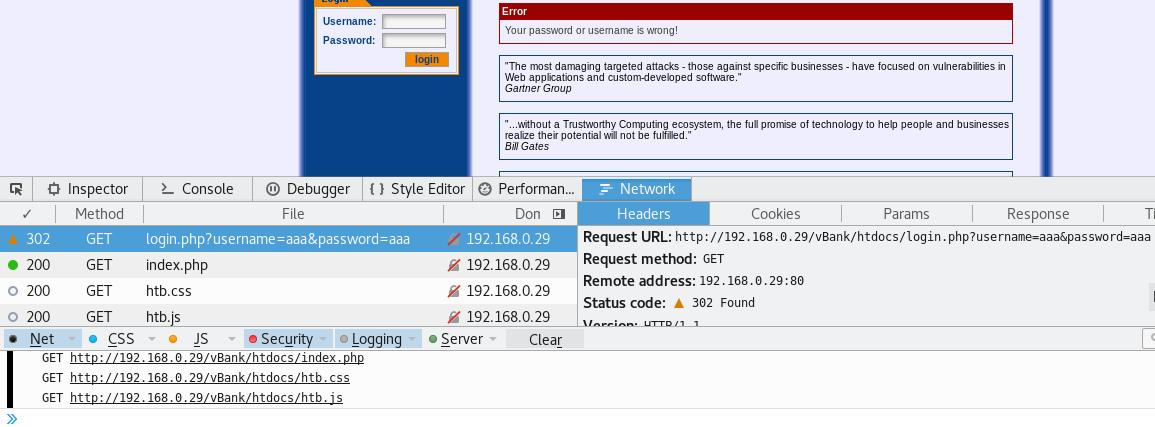
\includegraphics[width=0.75\textheight]{images/getmethod.jpg}
		\caption{Inspector panel in Firefox}
	\end{figure}
	Here we can see 'GET' method has been used to communicate with database, and the page is trying to open is 'login.php' with 'username=\&password=' parameter.\\
	If we put blank or wrong password, the error message would be 'your username or password is wrong'. Assuming the table's name is 'users', for the url: {\tt login.php?username=aaa\&password=aaa} will execute  sql query: {\sf SELECT * FROM users WHERE name='aaa' AND password='aaa'}.\\
	Now we will check if those parameters are accepting input through url. We run this: \\{\tt login.php?username=aaa\&password=aaa'} at later part of the url, and it give us a different error message: 'something went wrong during your attempt to login.', which means it is accepting input through url and thus the sql command became invalid like this:\\ {\sf SELECT * FROM users WHERE name='aaa' and password='aaa''}\\
	
	\paragraph*{2.} {\bf Fire your attack. Why is your attack successful? and what checks and mechanisms would prevent this failure (name at least two).}\\
	
	
	We can exploit further using this method. We can enter the system without knowing username or password. To enter the system, we just need to build a query such a way that the 'WHERE' condition becomes true. One possible option would be:\\ 
	{\tt login.php?username=aaa\&password=aaa'or 1=1}
	\\which executes this query: 
	\\{\sf SELECT * FROM users WHERE name='aaa' AND password='aaa' OR 1=1}
	\\Since 1=1 is always true, the query will be executed and returns the first row of 'users' table, where the first user 'alex' can be seen.
	\begin{figure}[H]
		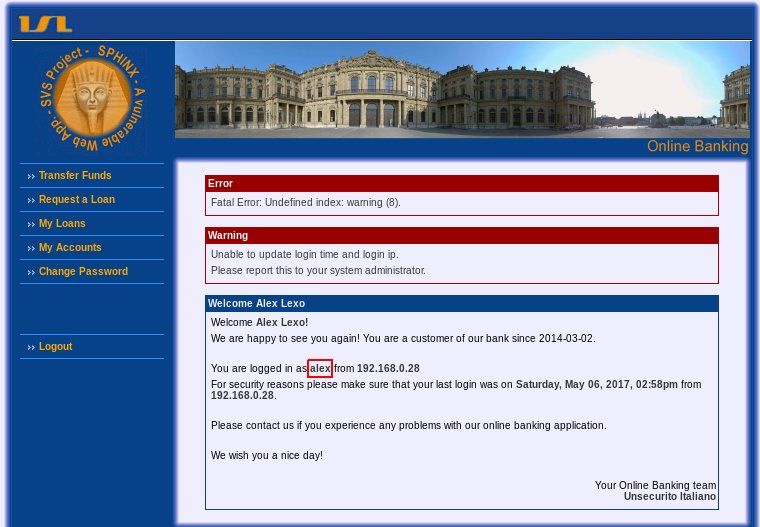
\includegraphics[width=0.75\textheight,height=0.4\textheight]{images/usernamefound.jpg}
		\caption{user 'alex' is found.}
	\end{figure}

	The attack was successful because the method of input handling on this web application is poorly developed. There is no validation or sanitation of input in the server side. Using latest web server and database could provide better security. Implementation of following could prevent this failure.
	\begin{itemize}
		\item using of prepared statement.
		\item using of stored procedure.
	\end{itemize}
	
	\paragraph*{3.} {\bf Change the password of the user you are logged in with. Briefly describe your actions and indicate the source code allowing for this attack.}\\
	Since we are logged in with user 'alex', it would be easy to change password. We navigate to 'change password' section. Here the old password is required in order to change. Since we do not know the password, we inspect the form, and found that this form is using 'POST' method, so we can use our queries in the old password textbox. We need to inject a query such a way that it results true. We use {\tt 'or'1=1} in the old password field and 'qqq' as new password. The system will show that the password is successfully changed.
	\begin{figure}[H]
		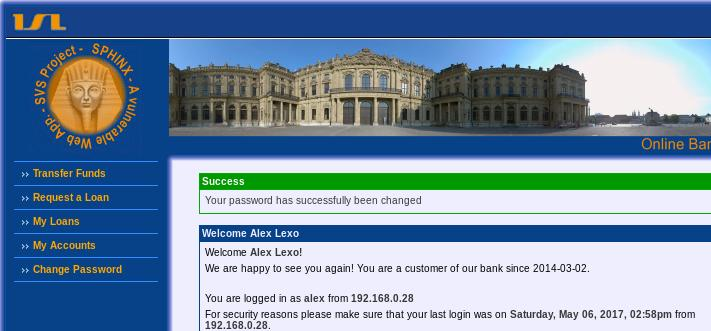
\includegraphics[width=0.75\textheight,height=0.3\textheight]{images/passsuccess.jpg}
		\caption{Password successful.}
	\end{figure}
	\begin{figure}[H]
		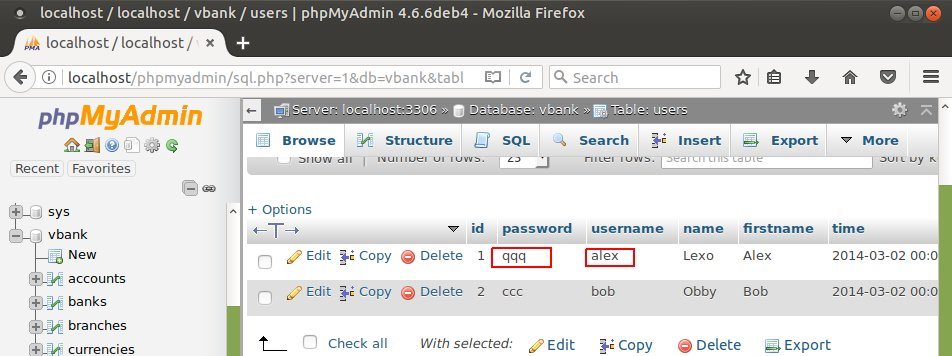
\includegraphics[width=0.75\textheight,height=0.2\textheight]{images/showpass.jpg}
		\caption{Password in the database.}
	\end{figure}
	
	\paragraph*{4.} {\bf Change the password of a known user (you know the login name of the user)!}\\
	In the case we know a username, let us assume the username is 'bob', we inject the following code in the later half of the url.\\
	{\sf login.php?username=bob\&password=\textasciiacute or \textasciiacute'='}\\
	This will give us access to as user bob.
	\begin{figure}[H]
		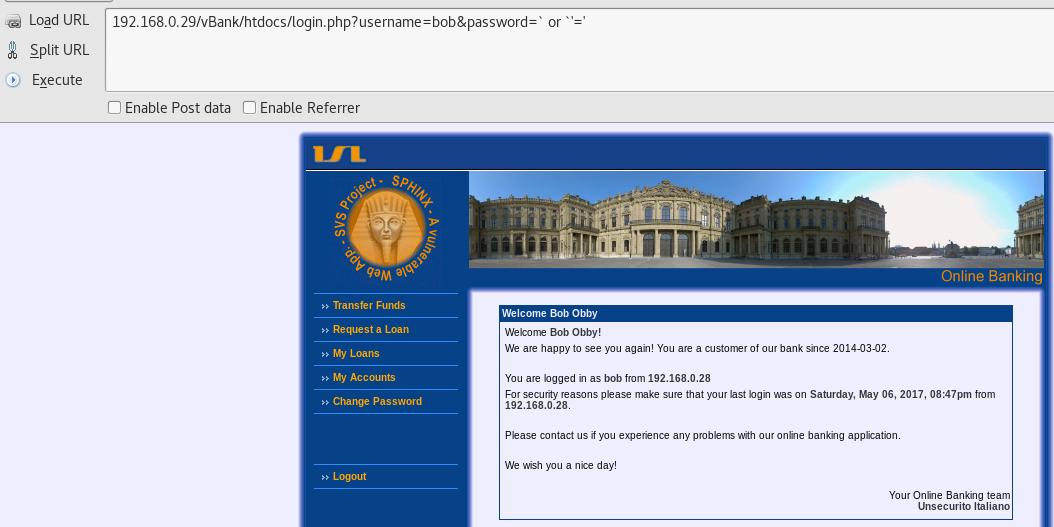
\includegraphics[width=0.75\textheight,height=0.3\textheight]{images/loginwithusername.jpg}
		\caption{Login with username: bob}
	\end{figure}
	To change the password we follow the steps described in 3.
	
	\newpage
	
	\section*{Exercise 4: SQL Injection - continued}
	In the last exercise you logged in without manipulating the attached database. Now you try to enter the bank without using the login-information of another person. Create your own account!
	\paragraph*{1.} {\bf Briefly describe how you retrieve the information you need to create a new user.}\\
	At the present stage we do not have any information about the database. Since our goal is to create our own account, we must know the database name, number of databse columns(number of tables) and the vulnerable column/s, and finally the table name and the column name where user's information is stored.\\
	First, we need to find out number columns(number of tables) and vulnerable columns of the database. We will continue injecting sql commands after putting a ' in the url. First, we try the following in the later part of the url.\\
	{\sf login.php?username=\&password=' or ' 1=1' order by 1 -{}-+}\\
	It will just login as alex will not show anything. Since it has logged in, which means our command is working. Now, with the 'order by' clause, we are trying to guessing the number of columns of the database. We will continue guessing by increasing the order by number. When we reach 'order by 9', it shows the following error:
	\begin{figure}[H]
		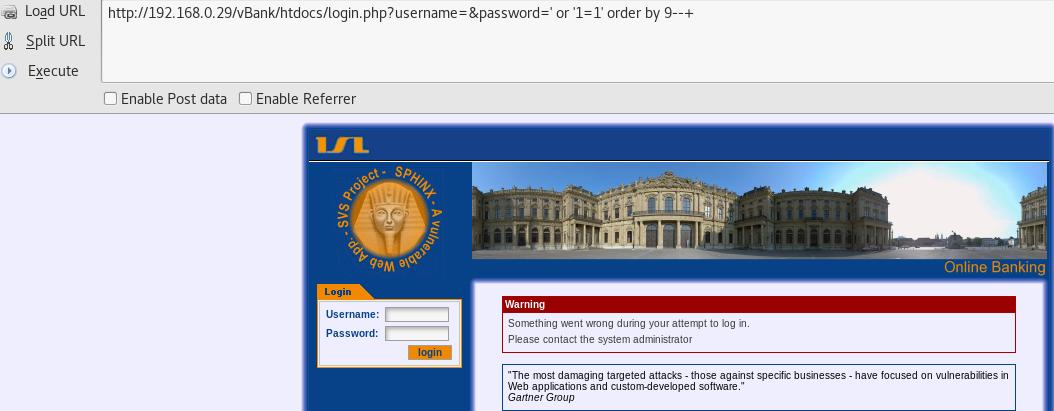
\includegraphics[width=0.75\textheight,height=0.3\textheight]{images/orderby.jpg}
		\caption{error in order by 9.}
	\end{figure}
	So, we can guess that, the database does not have 9th column, which means it has total 8 columns.\\
	We are going to find out which columns are vulnerable. In order to do that, we will inject {\tt UNION} operation of the sql in the url, as following:\\
	{\sf login.php?username=\&password=' UNION SELECT 1,2,3,4,5,6,7,8 -{}-+}\\
	We have not used anything in password field, and yet it has been logged in. Which means the query ran successfully. 
	\begin{figure}[H]
		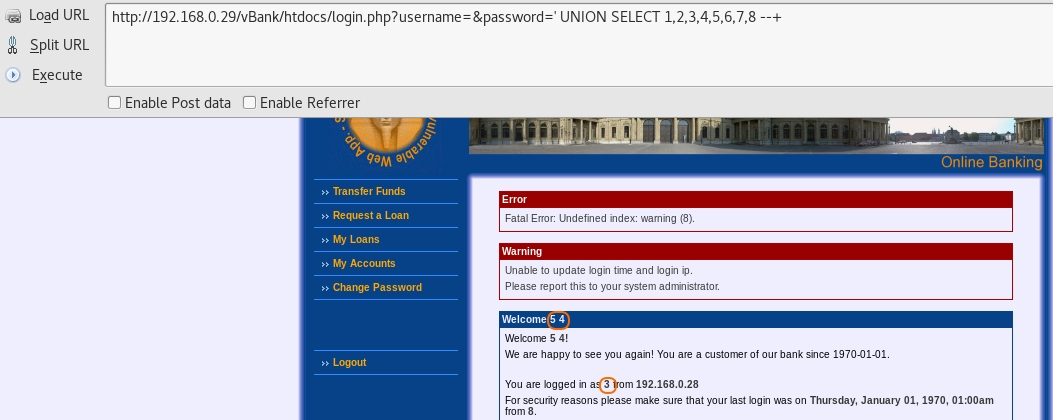
\includegraphics[width=0.75\textheight,height=0.3\textheight]{images/union1.jpg}
		\caption{Getting vulnerable columns.}
	\end{figure}
	The system has welcomed us as 3 5 and 4! which are the number of vulnerable columns, where we are going to exploit.\\
	Now we are going to retrieve the database name, injecting following command:\\
	{\sf login.php?username=\&password='UNION SELECT 1,2,database(),4,5,6,7,8 --+}\\
	Where {\sf databse() is a function which returns the name of database.}
	\begin{figure}[H]
		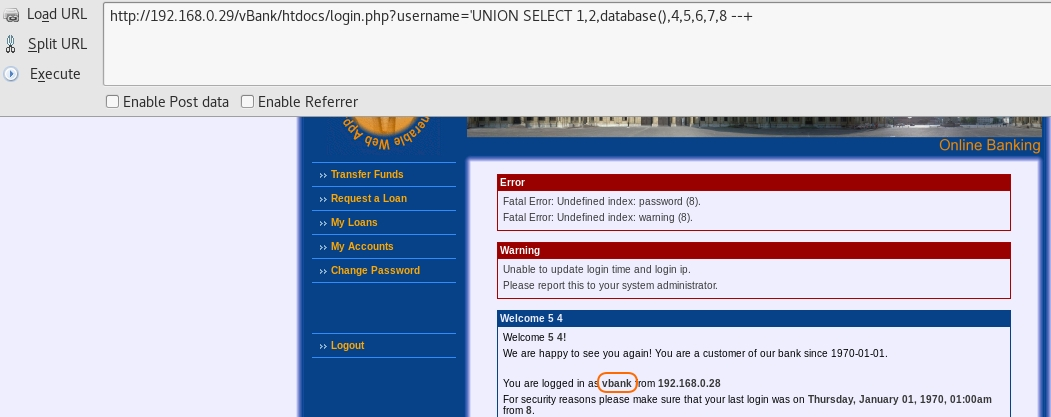
\includegraphics[width=0.7\textheight,height=0.25\textheight]{images/databasename.jpg}
		\caption{Name of the database found.}
	\end{figure}
	We found that, instead of 3, it is showing 'vbank' which is the name of database.\\
	In order to find out table names we inject following:\\
	\textsf{login.php?username=\&password'UNION SELECT 1, 2, group\_concat(TABLE\_NAME), 4, 5, 6, 7, 8 FROM information\_schema.tables WHERE table\_schema=database()-{}-+}
	\begin{figure}[H]
		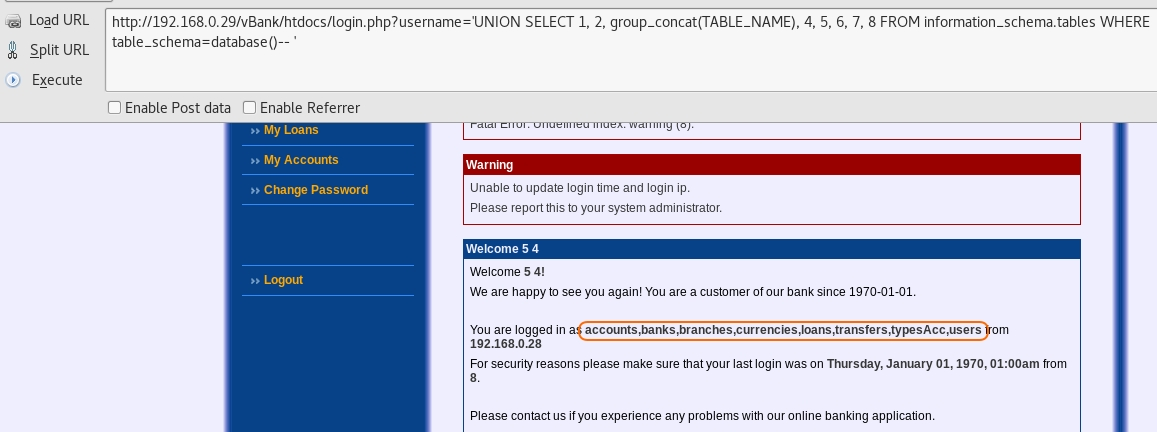
\includegraphics[width=0.75\textheight,height=0.3\textheight]{images/tablenames.jpg}
		\caption{Name of tables found.}
	\end{figure}
	Observing the tables, we can assume that the 'users' table has the information of users, and we are going to inject query for inserting users in this table.\\
	
	\paragraph*{2.} {\bf Briefly describe the actions required to create a new user.}
	Since we know the table to inject, we have to know the column names of this table by injecting following query:
	{\sf login.php?username=\&password=' UNION SELECT 1,2,group\_concat(column\_name),4,5,6,7,8 from information\_schema.columns where table\_name='users' -{}-+}
	It will return all the columns of users table:
	\begin{figure}[H]
		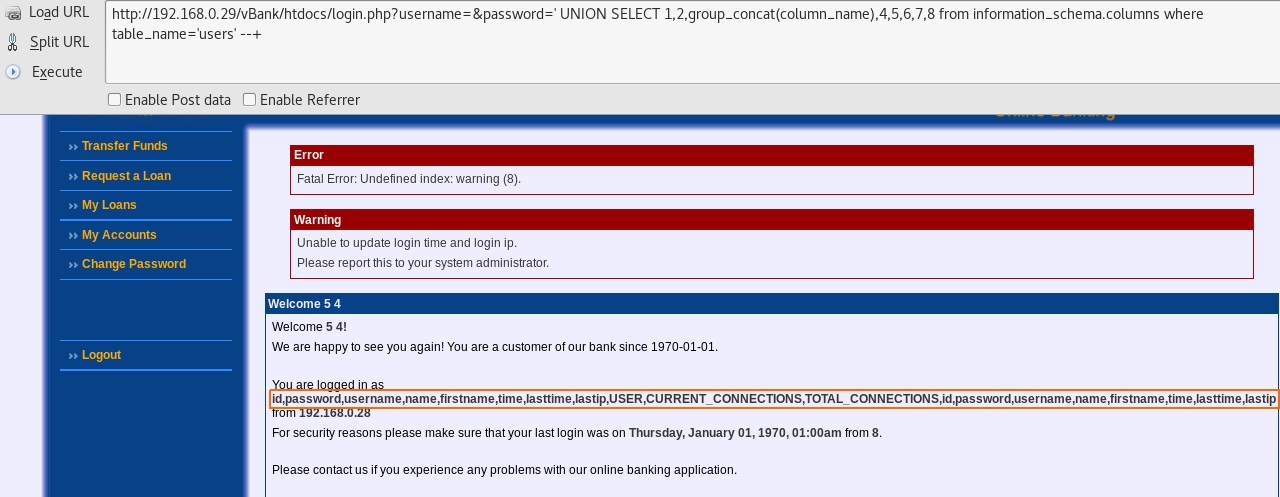
\includegraphics[width=0.75\textheight,height=0.3\textheight]{images/userscolumn.jpg}
		\caption{Name of columns of users table.}
	\end{figure}
	Now we have all the information to create our own user. It can be done by injecting {\sf INSERT INTO} clause.\\
	{\sf login.php?username=\&password='; INSERT INTO users (id,password,username,name,firstname) VALUES ('3','always','snape','snape','severus') -{}-+}\\
	Here is the screen shot of users table of the database.
	\begin{figure}[H]
		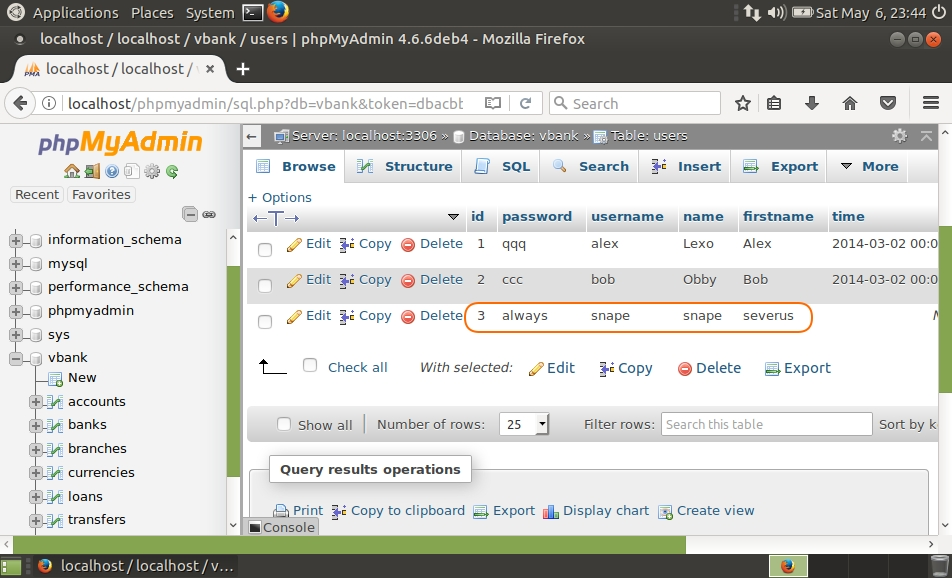
\includegraphics[width=0.75\textheight,height=0.3\textheight]{images/userinserted.jpg}
		\caption{A new user was inserted.}
	\end{figure}
	\paragraph*{3.} {\bf Give an additional precaution (apart from those you have given already) that may prevent this manipulation.}
	Previously we have mentioned following techniques to prevent this manipulation:
	\begin{itemize}
		\item Input sanitation.
		\item Using Stored procedure.
		\item Using Prepared Statemens.
		
	\end{itemize}
	The following additional precaution can be also considered to prevent sql injection.
	\begin{itemize}
		\item Escaping All User Supplied Input: to escape user input before putting it in a query. It is very database specific in its implementation.
		\item Least Privilege: minimize the privileges assigned to every database account in the environment. Prohibit to assign DBA or admin type access rights to the application accounts.
		\item Multiple DB Users: to avoid using the same admin account in the web applications to connect the database. Different DB users could be used for different web applications.
		\item Views: SQL views can further increase the granularity of access by limiting the read access to specific fields of a table or joins of tables.
	\end{itemize}
	


	
	
\end{document}